\section{BACKGROUND}
In this section, we review the MapReduce programming
model and describe the salient features of Phoenix, 
an implementation of MapReduce for multicore.
%讨论Phoenix的局限与不足

\subsection{MapReduce Programing Model}
The MapReduce programming model is inspired 
by funnctional languages and 
propose for data intensive computation in cluster environment.
It simple programming interface just require programmer 
defines two primitives: map and reduce.
The map function is applied on the input data and 
produces a list of intermediate key and value pairs.
The reduce function is applied on all intermediate
pairs and  groups all pairs with the same key to a single
key/value pair. 
The combine function is an aptional operation 
to aggregates the key and value pairs locally in Map Phase 
aiming to save networking bandwidth and reduce memory consumption.

The charm of MapReduce is that, for algorithms that
can fit that form, the library hides all the concurrency
from the programmer. For example, one can count the
number of occurrences of each word in a body of text as
follows. The map function emits a word, 1
pair for each word in document, and the reduce function counts
all occurrences of a word as the output. The combine function is
similar to the reduce function, but only processes a partial set of
key/value pairs.


\subsection{Phoenix}
Phoenix is an implementation of MapReduce for multicore 
and multiprocessor systems using Pthreads.
It shows MapReduce is a promising model 
and applications written with MapReduce model
have competitive scalability and performance with those
written with Pthreads\cite{ranger2007phoenix};

Phoenix stores the intermediate key/value pairs produced by the Map calls in a 
matrix(Figure \ref{fig:phoenix:intermediate}). 
Eche map and reduce workers can write or read the global buffer. 
Concurrent Map workers should avoid touching the same data.
To avoid locking and cache contention costs, when map workers
and reduce workes operate the buffer concurrently, there are two 
strategy must be done:\\
(1) Each row of the buffer is exclusively 
used by a worker in the Map phase, While each column of the buffer 
is exclusively used by a Phoenix Reduce worker. \\
(2) (To avoid map and reduce touching the same data), 
only When all map worker have been completed, 
Reduce worker begin working. 
There is a barrier between Map and Reduce phase.

\begin{figure}[!h!t]  
    \centering
    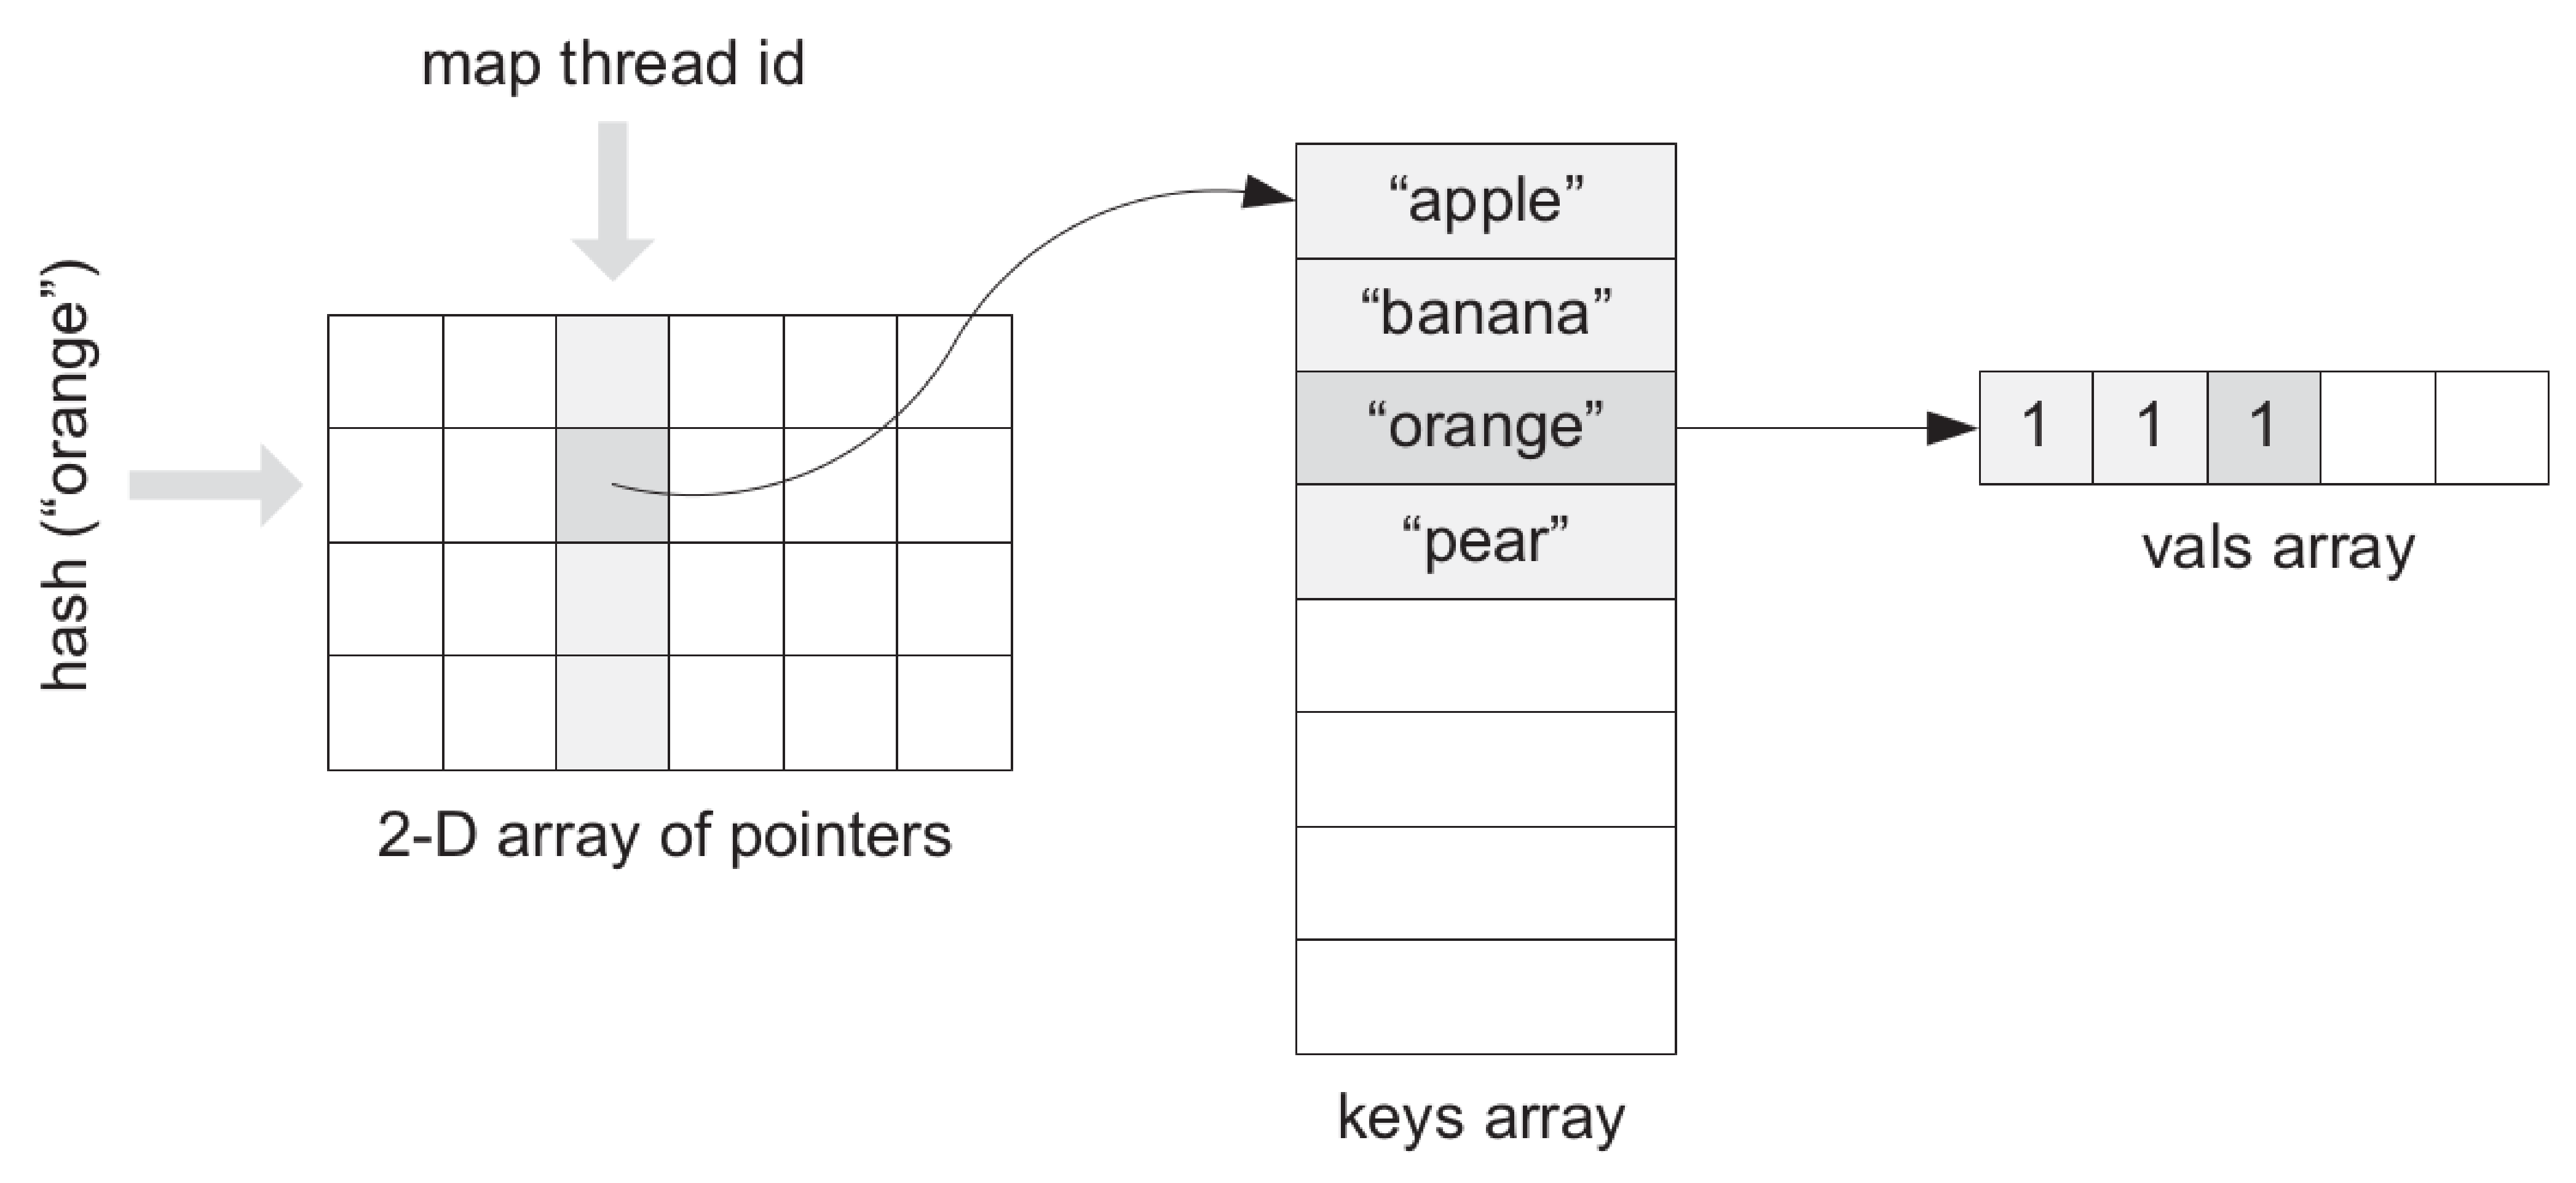
\includegraphics[width=0.45\textwidth]{eps/phoenix_intermediate.eps}
    \caption{Phoenix intermediate struct}
    \label{fig:phoenix:intermediate}
\end{figure}

As indicated in this figure\ref{fig:phoenix:speedup}, 
the Phoenix scales rather well when we use no more than four cores. 
However, when adding more cores in the system, 
the curve increases exponentially. 
The scalability of Phoenix is limited, the performance will be
better when the number of cores increases from 1 to 4, 
while the performance will be worse if using more than 4 cores. 
Perf\cite{} 


\begin{figure}[!h!t]  
    \centering
    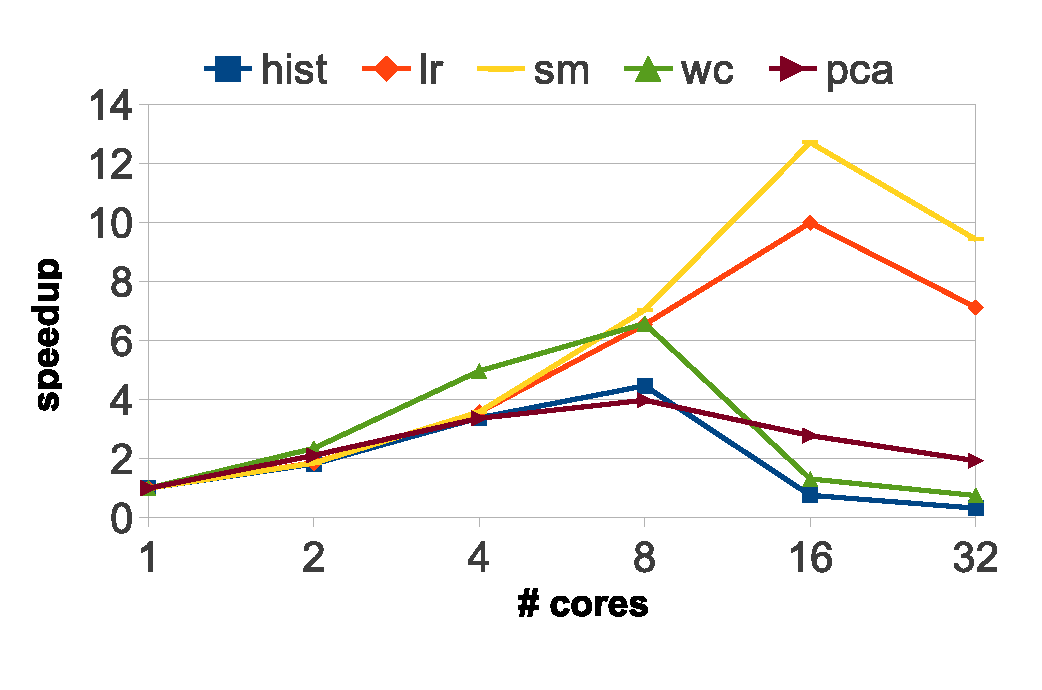
\includegraphics[width=0.45\textwidth]{eps/phoenix_speedup.eps}
    \caption{speedup of Phoenix}
    \label{fig:phoenix:speedup}
\end{figure}


\subsection{Optimizing Opportunities of Phoenix}
Though Phoenix has successfully demonstrated the feasibility
of running MapReduce applications on multicore, 
it also comes with some deficiencies 
{\color{gray}when processing jobs with a relatively large
amount of data, which would be common for machines with abundant memory and CPU cores
}.

First, there is a strict barrier between the Map and the Reduce phase, 
which requires workers in Reduce phase can only 
be startd until all workers in Map phase has been finished. 
Hence, the execution time of Map phase is determined by the slowest map worker.
If one of a map woker is slow, then the runtime of MapReduce will be need more time.
Futher, as the user-defined map functions are usually computation-intensive,
while the Reduce phase is memory-intensive,
the barrier is bad for the overall hardware resource utilization.
%barrier不利于资源的利用


Second, in cluster environments, 
the map tasks and reduce tasks are usually 
executed in different machines and data exchange among
tasks are done through networking, 
compared to shared memory in multicore environments. 
Hence, shared data structures , 
instead of networking communications, 
are the major performance bottlenecks processing large MapReduce jobs on multicore.
Multithreaded programs with hybrid shared mutable
data structures do not scale on multicore.
They suffer from serious lock contention.
Multithreaded applications on many-core processors can be
bottlenecked by contended locks inside the operating system’s
virtual memory system. 
Because of complex invariants in virtual memory systems, 
widely used in Linux kernels, 
have a single lock per shared address space. 
\cite{clements2013radixvm}


Phoenix do not achieve the desired scalability with increasing core count 
even with a simple, embarrassingly parallel job.
On a serious note, the internal
synchronization scheme (e.g., ticket spinlock) of
the virtualized instance on a machine with higher core count (e.g.,
32-core) dramatically degrades its overall performance.

{\color{red}our target of \myds}
%为了避免上述提到的问题,我们希望我们新设计的系统,拥有以下两个特性(1)break barrier (2),提升scalability



